\documentclass[a4paper,12pt]{article} 

% First, we usually want to set the margins of our document. For this we use the package geometry.
\usepackage[top = 2.5cm, bottom = 2.5cm, left = 2.5cm, right = 2.5cm]{geometry} 
\usepackage[T1]{fontenc}
\usepackage[utf8]{inputenc}

% The following two packages - multirow and booktabs - are needed to create nice looking tables.
\usepackage{multirow} % Multirow is for tables with multiple rows within one cell.
\usepackage{booktabs} % For even nicer tables.

% As we usually want to include some plots (.pdf files) we need a package for that.
\usepackage{graphicx} 

% The default setting of LaTeX is to indent new paragraphs. This is useful for articles. But not really nice for homework problem sets. The following command sets the indent to 0.
\usepackage{setspace}
\setlength{\parindent}{0in}

% Package to place figures where you want them.
\usepackage{float}

% The fancyhdr package let's us create nice headers.
\usepackage{fancyhdr}

\usepackage{amsmath,amsthm,tikz}

% To make our document nice we want a header and number the pages in the footer.

\pagestyle{fancy} % With this command we can customize the header style.

\fancyhf{} % This makes sure we do not have other information in our header or footer.

\lhead{\footnotesize Data Structure and Algorithm Analysis(H): Final Review}% \lhead puts text in the top left corner. \footnotesize sets our font to a smaller size.

%\rhead works just like \lhead (you can also use \chead)
\rhead{\footnotesize Mengxuan Wu} %<---- Fill in your lastnames.

% Similar commands work for the footer (\lfoot, \cfoot and \rfoot).
% We want to put our page number in the center.
\cfoot{\footnotesize \thepage} 

\begin{document}

\thispagestyle{empty} % This command disables the header on the first page. 

\begin{tabular}{p{15.5cm}}
{\large \bf Data Structure and Algorithm Analysis(H)} \\
Southern University of Science and Technology \\ Mengxuan Wu \\ 12212006 \\
\hline
\\
\end{tabular}

\vspace*{0.3cm} %add some vertical space in between the line and our title.

\begin{center}
	{\Large \bf Final Review}
	\vspace{2mm}

	{\bf Mengxuan Wu}
		
\end{center}  

\vspace{0.4cm}

\section{Sorting Algorithms} 

\subsection{Sorting Based on Comparison}

\subsubsection{Insertion Sort}

Inserting sort maintains a subarray of sorted element.
At each iteration, it inserts a new element into the subarray on the correct position.

\textbf{Runtime:} 
$\Omega(n)$, $O(n^2)$

\textbf{Correctness:} 
Proof by loop invariant: at the start of each iteration of the for loop, the subarray $A[1..j - 1]$ consists of the element originally in $A[1..j - 1]$, but in sorted order.

\textbf{Inplace:} 
Yes

\textbf{Stable:} 
Yes

\begin{center}
	\begin{tabular}{ll}
		\toprule
		\multicolumn{2}{l}{\textsc{Insertion-Sort}$(A)$} \\
		\midrule
		1. & \textbf{for} $j = 2$ to $A.length$ \\
		2. & \quad $key = A[j]$ \\
		3. & \quad $i = j - 1$ \\
		4. & \quad \textbf{while} $i > 0$ and $A[i] > key$ \\
		5. & \quad \quad $A[i + 1] = A[i]$ \\
		6. & \quad \quad $i = i - 1$ \\
		7. & \quad $A[i + 1] = key$ \\
		\bottomrule
	\end{tabular}
\end{center}

\subsubsection{Selection Sort}

Selection sort maintains a subarray of sorted element.
At each iteration, it selects the smallest element in the unsorted subarray, and swap it with the first element in the unsorted subarray.

\textbf{Runtime:} 
$\Theta(n^2)$

\textbf{Correctness:} 
Proof by loop invariant: at the start of each iteration of the for loop, the subarray $A[1..i - 1]$ consists of the $i - 1$ smallest elements.

\textbf{Inplace:} 
Yes

\textbf{Stable:}
No (example: $[2_a, 2_b, 1]$)

\begin{center}
	\begin{tabular}{ll}
		\toprule
		\multicolumn{2}{l}{\textsc{Selection-Sort}$(A)$} \\
		\midrule
		1. & \textbf{for} $i = 1$ to $A.length - 1$ \\
		2. & \quad $min = i$ \\
		3. & \quad \textbf{for} $j = i + 1$ to $A.length$ \\
		4. & \quad \quad \textbf{if} $A[j] < A[min]$ \\
		5. & \quad \quad \quad $min = j$ \\
		6. & \quad exchange $A[i]$ with $A[min]$ \\
		\bottomrule
	\end{tabular}
\end{center}

\subsubsection{Merge Sort}

Merge sort divides the array into two parts, sort each part recursively, and then merge the two sorted parts.

\textbf{Runtime:} 
$\Theta(n \log n)$

\textbf{Correctness:} 
\begin{itemize}
	\item Merge: By loop invariant: At the start of each iteration of the for loop, the subarray $A[p..k - 1]$ contains the $k - p$ smallest elements of $L[1..n_1 + 1]$ and $R[1..n_2 + 1]$, in sorted order.
	\item Merge sort: By induction: The two smaller subarrays are sorted correctly with induction hypothesis, and the merge step merges the two subarrays correctly.
\end{itemize}

\textbf{Inplace:}
No

\textbf{Stable:}
Yes

\begin{center}
	\begin{tabular}{rl}
		\toprule
		\multicolumn{2}{l}{\textsc{Merge}$(A, p, q, r)$} \\
		\midrule
		1. & $n_1 = q - p + 1$ \\
		2. & $n_2 = r - q$ \\
		3. & let $L[1 \dots n_1 + 1]$ and $R[1 \dots n_2 + 1]$ be new arrays \\
		4. & \textbf{for} $i = 1$ to $n_1$ \\
		5. & \quad $L[i] = A[p + i - 1]$ \\
		6. & \textbf{for} $j = 1$ to $n_2$ \\
		7. & \quad $R[j] = A[q + j]$ \\
		8. & $L[n_1 + 1] = \infty$ \\
		9. & $R[n_2 + 1] = \infty$ \\
		10. & $i = 1$ \\
		11. & $j = 1$ \\
		12. & \textbf{for} $k = p$ to $r$ \\
		13. & \quad \textbf{if} $L[i] \leq R[j]$ \\
		14. & \quad \quad $A[k] = L[i]$ \\
		15. & \quad \quad $i = i + 1$ \\
		16. & \quad \textbf{else} \\
		17. & \quad \quad $A[k] = R[j]$ \\
		18. & \quad \quad $j = j + 1$ \\
		\bottomrule
	\end{tabular}
\end{center}

\begin{center}
	\begin{tabular}{ll}
		\toprule
		\multicolumn{2}{l}{\textsc{Merge-Sort}$(A, p, r)$} \\
		\midrule
		1. & \textbf{if} $p < r$ \\
		2. & \quad $q = \lfloor (p + r) / 2 \rfloor$ \\
		3. & \quad \textsc{Merge-Sort}$(A, p, q)$ \\
		4. & \quad \textsc{Merge-Sort}$(A, q + 1, r)$ \\
		5. & \quad \textsc{Merge}$(A, p, q, r)$ \\
		\bottomrule
	\end{tabular}
\end{center}

\subsubsection{Heap Sort}

A heap is a binary tree with the following properties (assume the array starts from index 1):
\begin{enumerate}
	\item $A[Parent(i)] = \lfloor i / 2 \rfloor$.
	\item $A[Left(i)] = 2i$.
	\item $A[Right(i)] = 2i + 1$.
	\item Max-heap property: $A[Parent(i)] \geq A[i]$.
	\item Min-heap property: $A[Parent(i)] \leq A[i]$.
\end{enumerate}

\vspace{1cm}
\textbf{Max-heapify:}

Assume the binary trees rooted at $Left(i)$ and $Right(i)$ are max-heaps, but max-heap property may be violated at node $i$.
We let the value at node $i$ float down, so that the subtree rooted at node $i$ becomes a max-heap.

\textbf{Runtime:} 
$O(\log n)$ (height of the tree)

\textbf{Correctness:} 
By induction:
Assume max-heapify works for $h = i - 1$.
Now we consider $h = i$.
After we swap the value at node $i$ with the value at node $largest$, this maintains the max-heap property for node $i$.
Now one of the subtrees rooted at $Left(i)$ or $Right(i)$ may violate the max-heap property.
By induction hypothesis, we know that we can call max-heapify to make the subtree rooted at $Left(i)$ or $Right(i)$ a max-heap.

\begin{center}
	\begin{tabular}{rl}
		\toprule
		\multicolumn{2}{l}{\textsc{Max-Heapify}$(A, i)$} \\
		\midrule
		1. & $l = Left(i)$ \\
		2. & $r = Right(i)$ \\
		3. & \textbf{if} $l \leq A.heap-size$ and $A[l] > A[i]$ \\
		4. & \quad $largest = l$ \\
		5. & \textbf{else} $largest = i$ \\
		6. & \textbf{if} $r \leq A.heap-size$ and $A[r] > A[largest]$ \\
		7. & \quad $largest = r$ \\
		8. & \textbf{if} $largest \neq i$ \\
		9. & \quad exchange $A[i]$ with $A[largest]$ \\
		10. & \quad \textsc{Max-Heapify}$(A, largest)$ \\
		\bottomrule
	\end{tabular}
\end{center}

\vspace{1cm}
\textbf{Build-max-heap:}

Build-max-heap is used to build a max-heap from an unordered array.
We can only do bottom-up, since we need to maintain the max-heap property for all nodes.

\textbf{Runtime:} 
$O(n)$
The maximum number of nodes of height $h$ is $\lfloor n / 2^{h + 1} \rfloor$.
Hence, the total runtime is $\sum_{h = 0}^{\lfloor \log n \rfloor} \lfloor n / 2^{h + 1} \rfloor O(h) = O(n)$.

\textbf{Correctness:} 
By loop invariant:
At the start of each iteration of the for loop, each node $i + 1, i + 2, \dots, n$ have the max-heap property.

\begin{center}
	\begin{tabular}{rl}
		\toprule
		\multicolumn{2}{l}{\textsc{Build-Max-Heap}$(A)$} \\
		\midrule
		1. & $A.heap-size = A.length$ \\
		2. & \textbf{for} $i = \lfloor A.length / 2 \rfloor$ downto $1$ \\
		3. & \quad \textsc{Max-Heapify}$(A, i)$ \\
		\bottomrule
	\end{tabular}
\end{center}

\vspace{1cm}
\textbf{Heap-sort:}

We first build a max-heap from the array.
Then we can extract the maximum element from the heap, and put it at the end of the array.
Now we exchange the first element with the last element, decrease the heap size by 1, and call max-heapify to maintain the max-heap property.

\textbf{Runtime:}
$\Theta(n \log n)$

\textbf{Correctness:}
By loop invariant:
At the start of each iteration of the for loop, the subarray $A[1..i]$ is a max-heap that contains the first $i$ smallest elements, and the subarray $A[i + 1..n]$ contains the $n - i$ largest elements.

\textbf{Inplace:}
Yes

\textbf{Stable:}
No (example: $[1_a, 1_b]$)

\begin{center}
	\begin{tabular}{rl}
		\toprule
		\multicolumn{2}{l}{\textsc{Heap-Sort}$(A)$} \\
		\midrule
		1. & \textsc{Build-Max-Heap}$(A)$ \\
		2. & \textbf{for} $i = A.length$ downto $2$ \\
		3. & \quad exchange $A[1]$ with $A[i]$ \\
		4. & \quad $A.heap-size = A.heap-size - 1$ \\
		5. & \quad \textsc{Max-Heapify}$(A, 1)$ \\
		\bottomrule
	\end{tabular}
\end{center}

\subsubsection{Priority Queue}

A priority queue is very similar to a heap, but with the following operations:
\begin{enumerate}
	\item \textsc{Insert}$(Q, x)$: insert $x$ into $Q$.
	\item \textsc{Maximum}$(Q)$: return the element with the largest key.
	\item \textsc{Extract-Max}$(Q)$: remove and return the element with the largest key.
	\item \textsc{Increase-Key}$(Q, x, k)$: increase the key of $x$ to $k$.
\end{enumerate}

The only new operation is \textsc{Increase-Key}, which can be implemented by ``bubbling up'' the element.
Its runtime is $O(\log n)$.

\subsubsection{Quick Sort}

\textbf{Partition:}

Partition is used to partition an array into two parts, such that all elements in the first part are smaller than the pivot, and all elements in the second part are larger than the pivot.

\textbf{Runtime:} 
Worst case: $O(n^2)$, Best case: $O(n \log n)$, Average case: $O(n \log n)$

\textbf{Correctness:} 
By loop invariant: 
At the start of each iteration of the for loop, the subarray $A[p..j - 1]$ consists of elements smaller than the pivot, and the subarray $A[j + 1..r]$ consists of elements larger than the pivot.

\begin{center}
	\begin{tabular}{rl}
		\toprule
		\multicolumn{2}{l}{\textsc{Partition}$(A, p, r)$} \\
		\midrule
		1. & $x = A[r]$ \\
		2. & $i = p - 1$ \\
		3. & \textbf{for} $j = p$ to $r - 1$ \\
		4. & \quad \textbf{if} $A[j] \leq x$ \\
		5. & \quad \quad $i = i + 1$ \\
		6. & \quad \quad exchange $A[i]$ with $A[j]$ \\
		7. & exchange $A[i + 1]$ with $A[r]$ \\
		8. & \textbf{return} $i + 1$ \\
		\bottomrule
	\end{tabular}
\end{center}

\begin{center}
	\begin{tabular}{rl}
		\toprule
		\multicolumn{2}{l}{\textsc{Randomized-Partition}$(A, p, r)$} \\
		\midrule
		1. & $i = Random(p, r)$ \\
		2. & exchange $A[r]$ with $A[i]$ \\
		3. & \textbf{return} \textsc{Partition}$(A, p, r)$ \\
		\bottomrule
	\end{tabular}
\end{center}

However, there are some drawbacks of this implementation:
this partition algorithm behaves poorly if the input array contains many equal elements.

\vspace{1cm}
\textbf{Quick sort:}

Quick sort divides the array into two parts, and sort each part recursively.
It is very similar to merge sort, but it does not need to combine the two parts.

\textbf{Runtime:}
Worst case: $O(n^2)$, Best case: $O(n \log n)$, Average case: $O(n \log n)$

\textbf{Correctness:}
Similar to merge sort.
By induction, the two smaller subarrays are sorted correctly with induction hypothesis, and the partition step partitions the array correctly.

\textbf{Inplace:}
Yes

\textbf{Stable:}
No

\begin{center}
	\begin{tabular}{rl}
		\toprule
		\multicolumn{2}{l}{\textsc{Quick-Sort}$(A, p, r)$} \\
		\midrule
		1. & \textbf{if} $p < r$ \\
		2. & \quad $q = \textsc{Partition}(A, p, r)$ \\
		3. & \quad \textsc{Quick-Sort}$(A, p, q - 1)$ \\
		4. & \quad \textsc{Quick-Sort}$(A, q + 1, r)$ \\
		\bottomrule
	\end{tabular}
\end{center}

The randomized version is omitted here.

\vspace{1cm}
\textbf{Randomization:}

We can estimate the runtime of quick sort by the expected number of comparisons.

For a partition with fixed ratio, we can prove that the expected number of comparisons is always $O(n \log n)$.
Suppose the ratio is $1 : 9$, then we can draw a tree for the partition.
We can find at each level, if on both side all nodes exists, the number of comparisons is $n$.
And the maximum number of levels is $\log_{10/9} n$.
In total, the number of comparisons is $O(n \log n)$.

\vspace{1cm}
The expected number of comparisons for randomized quick sort can be calculated as follows:

Rename the array as $Z_1, Z_2, \dots, Z_n$, where $Z_1 < Z_2 < \dots < Z_n$.
Then the possibility that $Z_i$ is compared with $Z_j$ is $\frac{2}{j - i + 1}$ (suppose $i < j$).

Hence, the expected number of comparisons is:
\begin{equation*}
	\sum_{i = 1}^{n - 1} \sum_{j = i + 1}^{n} \frac{2}{j - i + 1} = \sum_{i = 1}^{n - 1} \sum_{k = 1}^{n - i} \frac{2}{k + 1} \leq \sum_{i = 1}^{n - 1} \sum_{k = 1}^{n - i} \frac{2}{k} \leq 2n \sum_{k = 2}^{n} \frac{1}{k} \leq 2n \ln n
\end{equation*}

\subsubsection{Lower Bound for Sorting Based on Comparison}

We can use decision tree to prove the lower bound for sorting.

Let the input size be $n$, suppose the input is a permutation of $1, 2, \dots, n$, there are $n!$ possible orders of the input.
Since each input must correspond to a leaf in the decision tree, the number of leaves is $n!$.
Hence, the height of the decision tree is $\Omega(\log n!)$.

The lower bound of worst case runtime is the length of the longest path in the decision tree, which is the height of the decision tree.
By Stirling's approximation, $\log n! = \Omega(n \log n)$.

\subsection{Sorting Based on Counting}

\subsubsection{Counting Sort}

Counting Sort assumes that each of the $n$ input elements is an integer in the range $0$ to $k$, for some integer $k$.
It works by counting the number of elements of each value.

\textbf{Runtime:} 
$\Theta(n + k)$

\textbf{Correctness:} 
By loop invariant:
At the start of each iteration of the for loop, the last element in $A$ with value $i$ that has not yet been copied to $B$ belongs to $B[C[i]]$.

\textbf{Inplace:}
No

\textbf{Stable:}
Yes

\begin{center}
	\begin{tabular}{rl}
		\toprule
		\multicolumn{2}{l}{\textsc{Counting-Sort}$(A, B, k)$} \\
		\midrule
		1. & let $C[0..k]$ be a new array \\
		2. & \textbf{for} $i = 0$ to $k$ \\
		3. & \quad $C[i] = 0$ \\
		4. & \textbf{for} $j = 1$ to $A.length$ \\
		5. & \quad $C[A[j]] = C[A[j]] + 1$ \\
		6. & \textbf{for} $i = 1$ to $k$ \\
		7. & \quad $C[i] = C[i] + C[i - 1]$ \\
		8. & \textbf{for} $j = A.length$ downto $1$ \\
		9. & \quad $B[C[A[j]]] = A[j]$ \\
		10. & \quad $C[A[j]] = C[A[j]] - 1$ \\
		\bottomrule
	\end{tabular}
\end{center}

\subsubsection{Radix Sort}

Radix Sort sorts the elements' digit by digit.

\textbf{Runtime:} 
$\Theta(d(n + k))$, where $d$ is the number of digits.

\textbf{Correctness:} 
At each iteration of the for loop, the elements are sorted on the last $i-1$ digits.

\textbf{Inplace:} 
No

\textbf{Stable:} 
Yes

\begin{center}
	\begin{tabular}{rl}
		\toprule
		\multicolumn{2}{l}{\textsc{Radix-Sort}$(A, d)$} \\
		\midrule
		1. & \textbf{for} $i = 1$ to $d$ \\
		2. & \quad use a stable sort to sort array $A$ on digit $i$ \\
		\bottomrule
	\end{tabular}
\end{center}

\textbf{Attention:} radix sort begins from the least significant digit.

When $d$ is a constant and $k = O(n)$, radix sort runs in $\Theta(n)$.
In more general cases, we can decide how to choose $d$ and $k$ to make the radix sort faster.

Without loss of generality, we assume the number is in base $2$.
The for a $b$ bit number, we can divide it into $\lceil b / d \rceil$ groups, each group has $d$ bits.
Then we can use counting sort to sort each group.
Hence, the runtime is $\Theta(\lceil b / d \rceil (n + 2^d))$.

When $b < \lfloor \log n \rfloor$, we can choose $d = b$.
Then the runtime is $\Theta(\frac{b}{b} (n + 2^b)) = \Theta(n)$.

When $b \geq \lfloor \log n \rfloor$, we can choose $d = \lfloor \log n \rfloor$.
Then the runtime is $\Theta(\frac{b}{\log n} (n + 2^{\log n})) = \Theta(\frac{bn}{\log n})$.


\section{Elementary Data Structures}

\subsection{Stack}

In a stack, only the top element can be accessed.
It follows the Last In First Out (LIFO) principle.

Its operations are:
\begin{enumerate}
	\item \textsc{Push}$(S, x)$: insert $x$ into $S$.
	\item \textsc{Pop}$(S)$: remove and return the top element of $S$.
\end{enumerate}

\textbf{Attention:} 
$S.top$ points at the top element of the stack, not an empty element.
We initialize $S.top = 0$.

\subsection{Queue}

In a queue, elements are inserted at the tail, and removed from the head.
A queue follows the First In First Out (FIFO) principle.

Its operations are:
\begin{enumerate}
	\item \textsc{Enqueue}$(Q, x)$: insert $x$ into $Q$.
	\item \textsc{Dequeue}$(Q)$: remove and return the head element of $Q$.
\end{enumerate}

\textbf{Attention:} 
$Q.head$ points at the head element of the queue, but $Q.tail$ points at the empty element after the tail element.
We initialize $Q.head = Q.tail = 1$.
It should be noted that a queue implemented in this way with an array of size $n$ can only store $n - 1$ elements.
Since if it stores $n$ elements, then $Q.head = Q.tail$, which means we cannot distinguish between an empty queue and a full queue.

\subsection{Linked List}

In a linked list, every element contains two pointers: one points at the previous element, and the other points at the next element.
It is also called a doubly linked list.

Linked list makes it easy to insert or delete an element.
Here are the pseudocode for insertion and deletion.

\begin{center}
	\begin{tabular}{rl}
		\toprule
		\multicolumn{2}{l}{\textsc{List-Insert}$(L, x)$} \\
		\midrule
		1. & $x.next = L.head$ \\
		2. & \textbf{if} $L.head \neq NIL$ \\
		3. & \quad $L.head.prev = x$ \\
		4. & $L.head = x$ \\
		5. & $x.prev = NIL$ \\
		\bottomrule
	\end{tabular}
\end{center}

\begin{center}
	\begin{tabular}{rl}
		\toprule
		\multicolumn{2}{l}{\textsc{List-Delete}$(L, x)$} \\
		\midrule
		1. & \textbf{if} $x.prev \neq NIL$ \\
		2. & \quad $x.prev.next = x.next$ \\
		3. & \textbf{else} $L.head = x.next$ \\
		4. & \textbf{if} $x.next \neq NIL$ \\
		5. & \quad $x.next.prev = x.prev$ \\
		\bottomrule
	\end{tabular}
\end{center}

\section{Binary Search Trees}

\subsection{General Binary Search Tree}

A binary search tree is a binary tree in which for each node $x$, the values of all the keys in the left subtree of $x$ are smaller than the key of $x$, and the values of all the keys in the right subtree of $x$ are larger than the key of $x$.

Here are some properties of a binary search tree:
\begin{itemize}
	\item The \textbf{depth} of a node $x$ is the number of edges on the simple path from the root to $x$. (Top Down)
	\item A level of a tree is all nodes at the same depth.
	\item The \textbf{height} of a node $x$ is the number of edges on the longest simple downward path from $x$ to a leaf. (Bottom Up)
	\item The height of a tree is the height of the root.
	\item A binary search tree is \textbf{full} if every node has either zero or two children.
	\item A binary search tree is \textbf{complete} if it is full and all leaves are at the same level.
\end{itemize}

\subsubsection{Successor}

The successor of a node $x$ is the node with the smallest key greater than $x.key$.
If a node has a right subtree, then its successor is the leftmost node in its right subtree.
If it does not, then its successor is the lowest ancestor of $x$ whose left child is also an ancestor of $x$.
Or to say, to find the first ``right parent'' of $x$.
Notice how this algorithm produce $NIL$ if $x$ is the largest node.

\begin{center}
	\begin{tabular}{rl}
		\toprule
		\multicolumn{2}{l}{\textsc{Tree-Successor}$(x)$} \\
		\midrule
		1. & \textbf{if} $x.right \neq NIL$ \\
		2. & \quad \textbf{return} \textsc{Tree-Minimum}$(x.right)$ \\
		3. & $y = x.p$ \\
		4. & \textbf{while} $y \neq NIL$ and $x = y.right$ \\
		5. & \quad $x = y$ \\
		6. & \quad $y = y.p$ \\
		7. & \textbf{return} $y$ \\
		\bottomrule
	\end{tabular}
\end{center}

The predecessor can be found similarly.

\subsubsection{Insert}

Insertion is simple, we do binary search to find a position, and then simply append the new node.
Notice that we want to keep record of the parent of current node, so that we can find the new node's parent.

\begin{center}
	\begin{tabular}{rl}
		\toprule
		\multicolumn{2}{l}{\textsc{Tree-Insert}$(T, z)$} \\
		\midrule
		1. & $x = T.root$ \\
		2. & $y = NIL$ \\
		3. & \textbf{while} $x \neq NIL$ \\
		4. & \quad $y = x$ \\
		5. & \quad \textbf{if} $z.key < x.key$ \\
		6. & \quad \quad $x = x.left$ \\
		7. & \quad \textbf{else} $x = x.right$ \\
		8. & $z.p = y$ \\
		9. & \textbf{if} $y = NIL$ \\
		10. & \quad $T.root = z$ \\
		11. & \textbf{else if} $z.key < y.key$ \\
		12. & \quad $y.left = z$ \\
		13. & \textbf{else} $y.right = z$ \\
		\bottomrule
	\end{tabular}
\end{center}

\subsubsection{Delete}

Deletion is more complicated.
We need to consider multiple cases:
\begin{enumerate}
	\item If $z$ is a leaf, we can simply remove it.
	\item If $z$ has only one child, we replace $z$ with its child.
	\item If $z$ has two children, we replace $z$ with its successor. 
	Why? Since the right subtree is not empty, the successor must be in the right subtree.
	The successor cannot have a left child, otherwise the left child will be the successor.
	Then we can replace $z$ with its successor, and then delete the successor (no left child makes it easy to delete).
	Since the successor has the smallest key that is larger than $z.key$, it is larger than all keys in the left subtree of $z$, and smaller than all keys in the right subtree of $z$.
	Then the binary search tree property is maintained.
\end{enumerate}

\begin{center}
	\begin{tabular}{rl}
		\toprule
		\multicolumn{2}{l}{\textsc{Tree-Delete}$(T, z)$} \\
		\midrule
		1. & \textbf{if} $z.left = NIL$ \\
		2. & \quad \textsc{Transplant}$(T, z, z.right)$ \\
		3. & \textbf{else if} $z.right = NIL$ \\
		4. & \quad \textsc{Transplant}$(T, z, z.left)$ \\
		5. & \textbf{else} \\
		6. & \quad $y = \textsc{Tree-Minimum}(z.right)$ \\
		7. & \quad \textbf{if} $y.p \neq z$ \\
		8. & \quad \quad \textsc{Transplant}$(T, y, y.right)$ \\
		9. & \quad \quad $y.right = z.right$ \\
		10. & \quad \quad $y.right.p = y$ \\
		11. & \quad \textsc{Transplant}$(T, z, y)$ \\
		12. & \quad $y.left = z.left$ \\
		13. & \quad $y.left.p = y$ \\
		\bottomrule
	\end{tabular}
\end{center}

\subsection{Tree Walk}

There are three ways to walk a tree:
\begin{enumerate}
	\item Preorder: root, left, right.
	\item Inorder: left, root, right.
	\item Postorder: left, right, root.
\end{enumerate}

Since it takes $\Theta(1)$ time to process each node, the runtime is $\Theta(n)$.

\begin{center}
	\begin{tabular}{rl}
		\toprule
		\multicolumn{2}{l}{\textsc{Inorder-Tree-Walk}$(x)$} \\
		\midrule
		1. & \textbf{if} $x \neq NIL$ \\
		2. & \quad \textsc{Inorder-Tree-Walk}$(x.left)$ \\
		3. & \quad print $x.key$ \\
		4. & \quad \textsc{Inorder-Tree-Walk}$(x.right)$ \\
		\bottomrule
	\end{tabular}
\end{center}

\begin{center}
	\begin{tabular}{rl}
		\toprule
		\multicolumn{2}{l}{\textsc{Preorder-Tree-Walk}$(x)$} \\
		\midrule
		1. & \textbf{if} $x \neq NIL$ \\
		2. & \quad print $x.key$ \\
		3. & \quad \textsc{Preorder-Tree-Walk}$(x.left)$ \\
		4. & \quad \textsc{Preorder-Tree-Walk}$(x.right)$ \\
		\bottomrule
	\end{tabular}
\end{center}

\begin{center}
	\begin{tabular}{rl}
		\toprule
		\multicolumn{2}{l}{\textsc{Postorder-Tree-Walk}$(x)$} \\
		\midrule
		1. & \textbf{if} $x \neq NIL$ \\
		2. & \quad \textsc{Postorder-Tree-Walk}$(x.left)$ \\
		3. & \quad \textsc{Postorder-Tree-Walk}$(x.right)$ \\
		4. & \quad print $x.key$ \\
		\bottomrule
	\end{tabular}
\end{center}

\subsection{AVL Trees}

A binary search tree can be unbalanced and degenerate into a linked list, which makes it inefficient.
An AVL tree is a self-balancing binary search tree.
It requires that the heights of the two child subtrees of any node differ by at most 1.
This can be implemented by adding a balance factor to each node.

An AVL tree with $n$ nodes has at most height $1.44 \log n$, which is pretty close to the optimal height $\log n$.

\subsubsection{Minimum Number of Nodes in AVL Tree}

Consider the minimal number of nodes in an AVL tree of height $h$.
We have:
\begin{equation*}
	N(h) = N(h - 1) + N(h - 2) + 1
\end{equation*}
This can be interpreted as: to find the minimal tree of height $h$, we split the AVL tree into three parts: the root, the left subtree of height $h - 1$, and the right subtree of height $h - 2$.
For the root, it satisfies the AVL property, since the height of the left subtree and the right subtree differ by 1.
For the two subtrees, to make the number of nodes minimal, they must be the minimal AVL trees of height $h - 1$ and $h - 2$.

This number is related to the Fibonacci sequence, and we have $N(h) = F_{h + 2} - 1$ (assume the Fibonacci sequence starts with $F_0 = F_1 = 1$).

\subsubsection{Insertion}

\textbf{Runtime:}
$O(\log n)$.

Firstly, we need to define the balance factor of a node $x$:
\begin{equation*}
	bal(x) = height(x.left) - height(x.right)
\end{equation*}

Without loss of generality, we assume the insertion inserts a node into the right subtree.
We use $v$ to denote the node on the path from the inserted node to the root, and $x$ to denote the right child of $v$.
Here are the cases:

\textbf{Case 1:} 
$bal(v) = 1$.
After insertion, $bal(v) = 0$.
The height of $v$ does not change, so we can stop.

\textbf{Case 2:}
$bal(v) = 0$.
After insertion, $bal(v) = -1$.
The height of $v$ increases by 1, so we need to check the parent of $v$, so we run the algorithm recursively.

\textbf{Case 3:}
$bal(v) = -1$.
After insertion, $bal(v) = -2$.
We need to do a rotation to make $v$ balanced.

\textbf{Subcase 3.1:}
The inserted node is in the right subtree of $x$.
We do a left rotation on $v$.
After the rotation, $v$ becomes the left child of $x$.
We then update the balance factor of $v$ and $x$: $bal(v) = 0$, $bal(x) = 0$.
Since the height of $v$ does not change, we can stop.

\textbf{Subcase 3.2:}
The inserted node is in the left subtree of $x$.
Let $w$ denote the left child of $x$.
We can find $v$, $x$, and $w$ form a zig-zag pattern.
We do a right rotation on $x$, and then a left rotation on $v$.
After the rotation, $v$ becomes the left child of $w$, and $x$ becomes the right child of $w$.
We then update the balance factor of $v$, $x$, and $w$:
\begin{itemize}
	\item If $bal(w)$ was 0, then $bal(v) = 0$, $bal(x) = 0$, $bal(w) = 0$.
	\item If $bal(w)$ was 1, then $bal(v) = 0$, $bal(x) = -1$, $bal(w) = 0$.
	\item If $bal(w)$ was -1, then $bal(v) = 1$, $bal(x) = 0$, $bal(w) = 0$.
\end{itemize}

\subsubsection{Deletion}

\textbf{Runtime:}
$O(\log n)$.

Deletion is similar to insertion.

Without loss of generality, we assume the deletion deletes a node from the left subtree.
We also need to consider three cases:

\textbf{Case 1:}
$bal(v) = 1$.
After deletion, $bal(v) = 0$.
The height of $v$ decreases by 1, so we need to check the parent of $v$, so we run the algorithm recursively.

\textbf{Case 2:}
$bal(v) = 0$.
After deletion, $bal(v) = 1$.
The height of $v$ does not change, so we can stop.

\textbf{Case 3:}
$bal(v) = -1$.
After deletion, $bal(v) = -2$.
We need to do a rotation to make $v$ balanced.

\textbf{Subcase 3.1:}
$bal(x) \in \{0, -1\}$.
The deleted node is in the left subtree of $v$.
We do a left rotation on $v$.
After the rotation, $v$ becomes the left child of $x$.
It depends on the balance factor of $x$ to decide whether we can stop.

\textbf{Subcase 3.2:}
$bal(x) = 1$.
The deleted node is in the left subtree of $v$.
Let $w$ denote the left child of $x$.
We do a right rotation on $x$, and then a left rotation on $v$.
After the rotation, $v$ becomes the left child of $w$, and $x$ becomes the right child of $w$.
The height of $v$ is decreased by 1, so we run the algorithm recursively.

\vspace{1cm}
It should be noted that if the deleted operation involves finding the successor, then we need to update the balance factor from the successor's parent.

\section{Dynamic Programming}

When we want to solve a problem recursively, we may find that some subproblems are solved repeatedly.
For example in the Fibonacci sequence, many numbers are calculated repeatedly.
So instead of solving the subproblems repeatedly, we can store the solutions in a table, and then use the table to solve the problem.

To implement dynamic programming, we often need the problem to be \textbf{optimal substructure} and \textbf{overlapping subproblems}.
\begin{itemize}
	\item Optimal substructure: The solution to the subproblem used within the optimal solution must be optimal.
	\item Overlapping subproblems: the problem can be broken down into subproblems which are reused several times.
\end{itemize}

\subsection{Rod Cutting}

Given a rod of length $n$ and a table of prices $p_i$ for the rod of length $i$, we want to find the maximum total revenue $r_n$ for the rod.
Let $r_i$ denote the maximum total revenue for the rod of length $i$.
Then we have the \textbf{Bellman equation}:
\begin{equation*}
	r_n = \max_{1 \leq i \leq n} (p_i + r_{n - i})
\end{equation*}

It should be noted that there is another Bellman equation, but we will not discuss it here:
\begin{equation*}
	r_n = \max (p_n, r_1 + r_{n - 1}, r_2 + r_{n - 2}, \dots, r_{n - 1} + r_1)
\end{equation*}

\subsubsection{Different Implementations}

\textbf{Recursive Implementation}

\begin{center}
	\begin{tabular}{rl}
		\toprule
		\multicolumn{2}{l}{\textsc{Cut-Rod}$(p, n)$} \\
		\midrule
		1. & \textbf{if} $n = 0$ \\
		2. & \quad \textbf{return} $0$ \\
		3. & $q = -\infty$ \\
		4. & \textbf{for} $i = 1$ to $n$ \\
		5. & \quad $q = \max(q, p_i + \textsc{Cut-Rod}(p, n - i))$ \\
		6. & \textbf{return} $q$ \\
		\bottomrule
	\end{tabular}
\end{center}

\textbf{Runtime:}
Let $T(n)$ denote the number of times \textsc{Cut-Rod} is called.
Then we have $T(n) = 1 + \sum_{i = 1}^{n} T(n - i)$.
Solve this recurrence relation, we have $T(n) = 2^n$.

\textbf{Bottom Up Implementation}

\begin{center}
	\begin{tabular}{rl}
		\toprule
		\multicolumn{2}{l}{\textsc{Bottom-Up-Cut-Rod}$(p, n)$} \\
		\midrule
		1. & $r_0 = 0$ \\
		2. & \textbf{for} $j = 1$ to $n$ \\
		3. & \quad $q = -\infty$ \\
		4. & \quad \textbf{for} $i = 1$ to $j$ \\
		5. & \quad \quad $q = \max(q, p[i] + r[j - i])$ \\
		6. & \quad $r[j] = q$ \\
		7. & \textbf{return} $r[n]$ \\
		\bottomrule
	\end{tabular}
\end{center}

In dynamic programming, correctly initializing the table is very important.
In this case, we initialize $r_0 = 0$.

\textbf{Runtime:}
$\Theta(n^2)$.

\textbf{Top Down Implementation}

This is also called \textbf{memoization}, we first check whether the subproblem has been solved, and if so, we return the solution.

\begin{center}
	\begin{tabular}{rl}
		\toprule
		\multicolumn{2}{l}{\textsc{Memoized-Cut-Rod}$(p, n)$} \\
		\midrule
		1. & \textbf{if} $r_n \geq 0$ \\
		2. & \quad \textbf{return} $r_n$ \\
		3. & $q = -\infty$ \\
		4. & \textbf{for} $i = 1$ to $n$ \\
		5. & \quad $q = \max(q, p_i + \textsc{Memoized-Cut-Rod}(p, n - i))$ \\
		6. & $r_n = q$ \\
		7. & \textbf{return} $q$ \\
		\bottomrule
	\end{tabular}
\end{center}

\textbf{Runtime:}
$\Theta(n^2)$.

It is worth noting that although in this particular case, the bottom up implementation is as fast as the top down implementation, in general, the memoization method is faster than the bottom up method.
This is because the memoization method only solves the subproblems that are needed, while the bottom up method solves all subproblems.

\subsection{Subproblem Graph}

We can draw a graph to show the subproblems and their dependencies.
For example, in the rod cutting problem, we can draw a graph as follows:
\begin{center}
	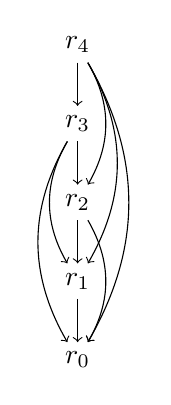
\begin{tikzpicture}
		\node (4) at (0, 0) {$r_4$};
		\node (3) at (0, -1) {$r_3$};
		\node (2) at (0, -2) {$r_2$};
		\node (1) at (0, -3) {$r_1$};
		\node (0) at (0, -4) {$r_0$};

		\draw[->] (4) edge (3);
		\draw[->] (4) edge[bend left] (2);
		\draw[->] (4) edge[bend left] (1);
		\draw[->] (4) edge[bend left] (0);
		\draw[->] (3) edge (2);
		\draw[->] (3) edge[bend right] (1);
		\draw[->] (3) edge[bend right] (0);
		\draw[->] (2) edge (1);
		\draw[->] (2) edge[bend left] (0);
		\draw[->] (1) edge (0);
	\end{tikzpicture}
\end{center}

When we estimate the runtime of a dynamic programming algorithm, it is often linear in the number of vertices and edges in the subproblem graph.

\subsection{Reconstruct The Solution}

In the rod cutting problem, we want to find the optimal solution, not just the optimal revenue.
We can use an auxiliary array $s$ to store the optimal size of the first piece to cut off.
Then we can reconstruct the solution by tracing back the array $s$.

For the bottom up implementation, we can implement a \textsc{Extended-Bottom-Up-Cut-Rod} to return both the optimal revenue and the auxiliary array $s$.
\begin{center}
	\begin{tabular}{rl}
		\toprule
		\multicolumn{2}{l}{\textsc{Extended-Bottom-Up-Cut-Rod}$(p, n)$} \\
		\midrule
		1. & $r_0 = 0$ \\
		2. & \textbf{for} $j = 1$ to $n$ \\
		3. & \quad $q = -\infty$ \\
		4. & \quad \textbf{for} $i = 1$ to $j$ \\
		5. & \quad \quad \textbf{if} $q < p_i + r_{j - i}$ \\
		6. & \quad \quad \quad $q = p_i + r_{j - i}$ \\
		7. & \quad \quad \quad $s_j = i$ \\
		8. & \quad $r_j = q$ \\
		9. & \textbf{return} $r_n, s$ \\
		\bottomrule
	\end{tabular}
\end{center}

Then we can print the solution by:
\begin{center}
	\begin{tabular}{rl}
		\toprule
		\multicolumn{2}{l}{\textsc{Print-Cut-Rod-Solution}$(p, n)$} \\
		\midrule
		1. & $(r, s) = \textsc{Extended-Bottom-Up-Cut-Rod}(p, n)$ \\
		2. & \textbf{while} $n > 0$ \\
		3. & \quad print $s[n]$ \\
		4. & \quad $n = n - s[n]$ \\
		\bottomrule
	\end{tabular}
\end{center}

\section{Greedy Algorithms}

A greedy algorithm always makes the choice that looks best at the moment.
A greedy algorithm always have a corresponding dynamic programming algorithm, but the converse is not true (otherwise we do not need dynamic programming).

\subsection{Activity Selection}

We have a set of activities $S = \{a_1, a_2, \dots, a_n\}$, where each activity $a_i$ has a start time $s_i$ and a finish time $f_i$.
Two activities $a_i$ and $a_j$ are \textbf{compatible} if $[s_i, f_i)$ and $[s_j, f_j)$ do not overlap.
The goal is to find the maximum-size subset of mutually compatible activities (\textbf{not the set of activities with the maximum total time}).

\subsubsection{Dynamic Programming}

We can use dynamic programming to solve this problem.
Let $S_{ij}$ denote the set of activities that start after $a_i$ finishes and finish before $a_j$ starts,
and let $A_{ij}$ denote the maximum-size subset of mutually compatible activities in $S_{ij}$.

The activity selection problem has optimal substructure:
Suppose $a_k$ is in $A_{ij}$, then $A_{ij} = A_{ik} \cup \{a_k\} \cup A_{kj}$.
Then $|A_{ij}| = |A_{ik}| + 1 + |A_{kj}|$.
Then we have the Bellman equation:
\begin{equation*}
	c[i, j] = \max_{a_k \in S_{ij}} (c[i, k] + c[k, j] + 1)
\end{equation*}

\subsubsection{Greedy Choice}

We can also use a greedy algorithm to solve this problem.
We first sort the activities by their finish time, and then we choose the first activity.
Then we choose the first activity that is compatible with the first activity, and so on.

In other words, we always choose the activity that finishes first.

Loop version:
\begin{center}
	\begin{tabular}{rl}
		\toprule
		\multicolumn{2}{l}{\textsc{Greedy-Activity-Selector}$(s, f)$} \\
		\midrule
		1. & $n = s.length$ \\
		2. & $A = \{a_1\}$ \\
		3. & $k = 1$ \\
		4. & \textbf{for} $m = 2$ to $n$ \\
		5. & \quad \textbf{if} $s_m \geq f_k$ \\
		6. & \quad \quad $A = A \cup \{a_m\}$ \\
		7. & \quad \quad $k = m$ \\
		8. & \textbf{return} $A$ \\
		\bottomrule
	\end{tabular}
\end{center}

Recursive version:
\begin{center}
	\begin{tabular}{rl}
		\toprule
		\multicolumn{2}{l}{\textsc{Recursive-Activity-Selector}$(s, f, k, n)$} \\
		\midrule
		1. & $m = k + 1$ \\
		2. & \textbf{while} $m \leq n$ and $s_m < f_k$ \\
		3. & \quad $m = m + 1$ \\
		4. & \textbf{if} $m \leq n$ \\
		5. & \quad \textbf{return} $\{a_m\} \cup \textsc{Recursive-Activity-Selector}(s, f, m, n)$ \\
		6. & \textbf{else} \\
		7. & \quad \textbf{return} $\emptyset$ \\
		\bottomrule
	\end{tabular}
\end{center}

\textbf{Runtime:}
$\Theta(n)$.

\subsubsection{Proof of Correctness}

We assume that the activities are sorted by their finish time.
Let $S_k$ denote the set of activities the starts after $a_k$ finishes, and $A_k$ denote the maximum-size subset of mutually compatible activities in $S_k$.
We want to prove that if $a_m$ is the activity that finishes first in the set $S_k$, then $a_k$ is in some $A_k$.

Let $a_j$ denote the activity that finishes first in $A_k$.
If $a_j = a_m$, then we are done.
If $a_j \neq a_k$, we can exchange $a_j$ and $a_m$ and not cause any conflict.
Since the number of activities in $A_k$ does not change, the new set is still a maximum-size subset of mutually compatible activities in $S_k$.

\subsection{General Scheme of Greedy Algorithms}

\begin{enumerate}
	\item Cast the optimization problem as one in which we make a choice and are left with one subproblem to solve.
	\item Prove that there is always an optimal solution to the original problem that makes the greedy choice, so that the greedy choice is always safe.
\end{enumerate}

\subsection{Coin Changing}

Given a set of coins $S = \{v_1, v_2, \dots, v_n\}$, where $v_1 < v_2 < \dots < v_n$, and a value $V$, we want to find the minimum number of coins that sum to $V$.
This problem does not always have a greedy solution.

The usual greedy choice is to choose the largest coin that does not exceed the remaining value.
This sometimes fails, for example: $S = \{1, 3, 4\}$, $V = 6$.
The greedy algorithm will choose $4, 1, 1$, but the optimal solution is $3, 3$.

\subsection{When Greedy Algorithms Fail}

There are many cases when greedy algorithms fail.
For example: maze problem, traveling salesman problem, 0-1 knapsack problem, etc.

Take 0-1 knapsack problem as an example.
If we have a knapsack with capacity 50 and three items:
\begin{itemize}
	\item Item 1: $v_1 = 60$, $w_1 = 10$
	\item Item 2: $v_2 = 100$, $w_2 = 20$
	\item Item 3: $v_3 = 120$, $w_3 = 30$
\end{itemize}

If the greedy choice is to choose the item with the largest value per unit weight, then we will choose item 1 and 2, and the total value is 160.
However, the optimal solution is to choose item 2 and 3, and the total value is 220.

It should be noted that the \textbf{fractional knapsack problem} does have a greedy solution.

\section{Graph Algorithms}

We usually use two ways to represent a graph: adjacency list and adjacency matrix.
To choose which representation to use, we need to consider the density of the graph.
A graph is \textbf{sparse} if $|E| = o(|V|^2)$, and \textbf{dense} if $|E| = \Theta(|V|^2)$.
For sparse graphs, we use adjacency list, and for dense graphs, we use adjacency matrix.

\subsection{Breadth First Search}

In breadth first search, we use a queue to store the vertices.
We extract a vertex from the queue, and then add all its adjacent vertices to the queue.

We assign each vertex a color: white, gray, or black.
\begin{itemize}
	\item White: undiscovered.
	\item Gray: discovered but not finished.
	\item Black: finished.
\end{itemize}
\textit{It is worth noting that the two colors gray and black are not necessary and can be combined into one color.
The difference is purely for the purpose of analysis.}

Each vertex has three attributes: distance, parent, and color.

\begin{center}
	\begin{tabular}{rl}
		\toprule
		\multicolumn{2}{l}{\textsc{BFS}$(G, s)$} \\
		\midrule
		1. & \textbf{for} each vertex $u \in G.V - \{s\}$ \\
		2. & \quad $u.color = WHITE$ \\
		3. & \quad $u.d = \infty$ \\
		4. & \quad $u.\pi = NIL$ \\
		5. & $s.color = GRAY$ \\
		6. & $s.d = 0$ \\
		7. & $s.\pi = NIL$ \\
		8. & $Q = \emptyset$ \\
		9. & \textsc{Enqueue}$(Q, s)$ \\
		10. & \textbf{while} $Q \neq \emptyset$ \\
		11. & \quad $u = \textsc{Dequeue}(Q)$ \\
		12. & \quad \textbf{for} each vertex $v \in G.Adj[u]$ \\
		13. & \quad \quad \textbf{if} $v.color == WHITE$ \\
		14. & \quad \quad \quad $v.color = GRAY$ \\
		15. & \quad \quad \quad $v.d = u.d + 1$ \\
		16. & \quad \quad \quad $v.\pi = u$ \\
		17. & \quad \quad \quad \textsc{Enqueue}$(Q, v)$ \\
		18. & \quad $u.color = BLACK$ \\
		\bottomrule
	\end{tabular}
\end{center}

\textbf{Runtime:}
$O(|V| + |E|)$.
This is because each vertex is enqueued and dequeued at most once, which takes $O(|V|)$ time.
Each edge is examined at most twice, which takes $O(|E|)$ time (assume we use adjacency list).

\textbf{Correctness:}
The loop invariant is: 
At the start of each iteration of the while loop, the queue $Q$ contains all the vertices that are gray.
However by the loop invariant only, we cannot prove the correctness of the algorithm.

We can prove the correctness by using the following facts:
\begin{itemize}
	\item \textit{Let the length of the shortest path from $s$ to $u$ be $d(s, u)$.
		Then for a graph $G = (V, E)$, if an edge $(u, v) \in E$, then $d(s, v) \leq d(s, u) + 1$.}
		This is true because the shortest path from $s$ to $v$ cannot be longer than the shortest path from $s$ to $u$ plus the edge $(u, v)$.
	\item \textit{When the breadth first search ends, for each vertex $v \in V$, $v.d \geq d(s, v)$.}
		This can be proved by induction.
		The base case is trivial.
		For the inductive step, we can find on line 15 that $v.d = u.d + 1$.
		Together with the fact that $u.d \geq d(s, u)$, we have $v.d = u.d + 1 \geq d(s, u) + 1 \geq d(s, v)$.
	\item \textit{Suppose the first vertex in the queue is $v_1$ and the last vertex in the queue is $v_k$.
		Then for each $i = 2, 3, \dots, k$, $v_i.d \geq v_{i - 1}.d$ and $v_k.d \leq v_1.d + 1$.}
		This can be proved by induction.
		The base case is trivial.
		When we dequeue $v_1$, by the inductive hypothesis, we have $v_2.d \geq v_1.d$.
		Then we can find $v_k.d \leq v_1.d + 1 \leq v_2.d + 1$.
		When we enqueue $v_{k+1}$, let the current processing vertex be $u$.
		By the inductive hypothesis, we have $v_{k + 1}.d = u.d + 1 \leq v_1.d + 1$.
		Also, $v_k \leq u.d + 1 = v_{k + 1}.d$.
	\item \textit{Suppose $v_i$ and $v_j$ are two vertices in the queue, and $v_i$ is enqueued before $v_j$.
		Then $v_i.d \leq v_j.d$.}
		This can be proved by the last fact.
	\item \textit{If $v$ and $u$ are neighbors, then $v.d \leq u.d + 1$.}
		When $u$ is dequeued:
		\begin{itemize}
			\item If $v$ is white, then $v$ is enqueued, and $v.d = u.d + 1$.
			\item If $v$ is gray, then by fact 3, $v.d \leq u.d + 1$.
			\item If $v$ is black, then $v$ is enqueued before $u$, and by fact 4, $v.d \leq u.d$.
		\end{itemize}
	\item \textit{After the breadth first search ends, for each vertex $v \in V$, $v.d$ is the shortest path from $s$ to $v$.}
		This can be proved by contradiction.
		Suppose a vertex $v$ has a shorter path from $s$ to $v$, or to say $v.d > d(s, v)$, and $v$ has the shortest mismatched path.
		Then let vertex $u$ be the last vertex on the shortest path from $s$ to $v$.
		By the choice of $v$, we have $u.d + 1  = d(s, u) + 1 = d(s, v) < v.d$.
		By fact 5, we have $v.d \leq u.d + 1$, which contradicts the previous inequality.
\end{itemize}

\vspace{1cm}
The shortest path can be found by tracing back the parent pointers.
This means the breadth first search tree is a shortest path tree, and is a single source shortest path algorithm.

\subsection{Depth First Search}

In depth first search, we use a stack to store the vertices.
Each vertex has four attributes: discovery time, finish time, parent, and color.

\begin{center}
	\begin{tabular}{rl}
		\toprule
		\multicolumn{2}{l}{\textsc{DFS}$(G)$} \\
		\midrule
		1. & \textbf{for} each vertex $u \in G.V$ \\
		2. & \quad $u.color = WHITE$ \\
		3. & \quad $u.\pi = NIL$ \\
		4. & $time = 0$ \\
		5. & \textbf{for} each vertex $u \in G.V$ \\
		6. & \quad \textbf{if} $u.color == WHITE$ \\
		7. & \quad \quad \textsc{DFS-Visit}$(G, u)$ \\
		\bottomrule
	\end{tabular}
\end{center}

\begin{center}
	\begin{tabular}{rl}
		\toprule
		\multicolumn{2}{l}{\textsc{DFS-Visit}$(G, u)$} \\
		\midrule
		1. & $time = time + 1$ \\
		2. & $u.d = time$ \\
		3. & $u.color = GRAY$ \\
		4. & \textbf{for} each vertex $v \in G.Adj[u]$ \\
		5. & \quad \textbf{if} $v.color == WHITE$ \\
		6. & \quad \quad $v.\pi = u$ \\
		7. & \quad \quad \textsc{DFS-Visit}$(G, v)$ \\
		8. & $u.color = BLACK$ \\
		9. & $time = time + 1$ \\
		10. & $u.f = time$ \\
		\bottomrule
	\end{tabular}
\end{center}

\textbf{Runtime:}
$O(V + E)$.
Each vertex is discovered and finished exactly once, and each edge is examined exactly twice.

\subsubsection{Properties of Depth First Search}

\begin{itemize}
	\item \textbf{Parenthesis property:}
	For any two vertices $u$ and $v$, exactly one of the following three conditions holds:
	\begin{itemize}
		\item The intervals $[u.d, u.f]$ and $[v.d, v.f]$ are entirely disjoint, and neither $u$ nor $v$ is a descendant of the other in the depth first forest.
		\item The interval $[u.d, u.f]$ is contained entirely within the interval $[v.d, v.f]$, and $u$ is a descendant of $v$ in a depth first tree.
		\item The interval $[v.d, v.f]$ is contained entirely within the interval $[u.d, u.f]$, and $v$ is a descendant of $u$ in a depth first tree.
	\end{itemize}
	\item \textbf{White-path theorem:}
	In a depth first forest of a graph $G = (V, E)$, vertex $v$ is a descendant of vertex $u$ if and only if at the time $u.d$ that the search discovers $u$, there is a path from $u$ to $v$ consisting entirely of white vertices.
\end{itemize}

\textbf{Proof:}

``$\Rightarrow$'':
If $v$ is a descendant of $u$, then $v$ is discovered after $u$, which means $v$ is white when $u$ is discovered.
And this is true for all vertices on the path from $u$ to $v$, since they are all descendants of $u$.

``$\Leftarrow$'':
Proof by contradiction.
Let $v$ be the first vertex on the white path but is not a descendant of $u$.
Let $w$ be the predecessor of $v$ on the white path.
By the choice of $w$, we knoe that $w$ is a descendant of $u$, hence $u.d \leq w.f \leq u.f$. ($w$ and $u$ can be the same vertex.)
Since there is a path from $w$ to $v$, $v$ will be discovered before $w$ finishes, hence $v.d < w.f$.
In all, we have $u.d < v.d < w.f \leq u.f$, then $v$ must be a descendant of $u$.

\subsubsection{Classification of Edges}

There are four types of edges in a depth first forest:
\begin{itemize}
	\item \textbf{Tree edges:}
	Edges in the depth first forest.
	An edge $(u, v)$ is a tree edge if $v$ was first discovered by exploring edge $(u, v)$, or to say $v$'s color is white when edge $(u, v)$ is examined.
	\item \textbf{Back edges:}
	Edges that connect a vertex to an ancestor in a depth first tree.
	An edge $(u, v)$ is a back edge if at the time $(u, v)$ is examined, $v$ is colored gray.
	\item \textbf{Forward edges:}
	Edges that connect a vertex to a descendant in a depth first tree.
	An edge $(u, v)$ is a forward edge if at the time $(u, v)$ is examined, $v$ is colored black and was discovered later than $u$.
	\item \textbf{Cross edges:}
	Edges that connect two vertices in different depth first trees.
	An edge $(u, v)$ is a cross edge if at the time $(u, v)$ is examined, $v$ is colored black and was discovered earlier than $u$.
\end{itemize}

In an undirected graph, there are only tree edges and back edges.
This is because there is no way to find a vertex that is colored black.

Let $(u,v)$ be an arbitrary edge of an undirected graph $G = (V, E)$.
Without loss of generality, assume that $u.d < v.d$.
Hence, the search must discover $v$ before it finishes exploring $u$.
If the first time that $(u, v)$ is examined is from $u$, then it is a tree edge.
Otherwise, $(u, v)$ is a back edge, since $u$ is still gray when $(u, v)$ is examined.

\subsubsection{DFS and Cycle}

A directed graph is acyclic if and only if a depth first search of the graph yields no back edges.

\textbf{Proof:}

``$\Leftarrow$'':
If there is a back edge $(u, v)$, then we can find a loop that consists of a path from $u$ to $v$ on the depth first tree, and the edge $(u, v)$.

``$\Rightarrow$'':
If there is a loop, then there is a back edge.
Assume the cycle is $v_1, v_2, \dots, v_k, v_1$.
Without loss of generality, assume the first discovered vertex is $v_1$.
Then at time $v_1.d$, all other vertices are colored white.
By the white-path theorem, $v_k$ is a descendant of $v_1$.
Therefore, $(v_1, v_k)$ is a back edge.

\subsubsection{Topological Sort}

A topological sort of a directed acyclic graph $G = (V, E)$ is a linear ordering of all its vertices such that if $G$ contains an edge $(u, v)$, then $u$ appears before $v$ in the ordering.
A topological sort can be implemented by depth first search.

\begin{center}
	\begin{tabular}{rl}
		\toprule
		\multicolumn{2}{l}{\textsc{Topological-Sort}$(G)$} \\
		\midrule
		1. & \textbf{call} \textsc{DFS}$(G)$ to compute finishing times $v.f$ for each vertex $v$ \\
		2. & \textbf{as each vertex is finished, insert it onto the front of a linked list} \\
		3. & \textbf{return} the linked list of vertices \\
		\bottomrule
	\end{tabular}
\end{center}

\textbf{Runtime:}
$O(|V| + |E|)$.

\textbf{Correctness:}
For any edge $(u, v)$, we need to prove that $u.f > v.f$.
Without loss of generality, assume $u$ is discovered before $v$.
Since in an acyclic graph there is no back edge, $v$ must be white or black.
If $v$ is white, then $v$ is a descendant of $u$, and $u.f > v.f$.
If $v$ is black, then $v.f$ is already set and $u.f > v.f$.

\subsubsection{Strongly Connected Components}

A directed graph is \textbf{strongly connected} if there is a path from each vertex to every other vertex.
Let $G = (V, E)$ be a directed graph, and let $G^T = (V, E^T)$ be the transpose of $G$, which is the graph formed by reversing all edges in $G$.
Note that $G$ and $G^T$ have the same strongly connected components.

\begin{center}
	\resizebox{\linewidth}{!}{
		\begin{tabular}{rl}
			\toprule
			\multicolumn{2}{l}{\textsc{Strongly-Connected-Components}$(G)$} \\
			\midrule
			1. & \textbf{call} \textsc{DFS}$(G)$ to compute finishing times $u.f$ for each vertex $u$ \\
			2. & \textbf{compute} $G^T$ \\
			3. & \textbf{call} \textsc{DFS}$(G^T)$, but in the main loop of \textsc{DFS}, consider the vertices in order of decreasing $u.f$ \\
			4. & \textbf{output} the vertices of each tree in the depth first forest formed in line 3 as a separate strongly connected component \\
			\bottomrule
		\end{tabular}
	}
\end{center}

\textbf{Runtime:}
$O(|V| + |E|)$

\textbf{Correctness:}
Proof by induction.
An SCC must be in its own tree in the depth first forest.
And we know the SCC containing the root of a depth first tree can be correctly output.
Then we make induction on the number of SCC in the graph.
If there is only one SCC, then the algorithm is correct (it will contain the root of the depth first tree).
Then, if we want to output the SCCs of a graph with $k$ SCCs, we can exclude the SCC containing the root of one depth first tree, and output the SCCs of the remaining graph, which has $k - 1$ SCCs.

\subsection{Minimum Spanning Tree}

A \textbf{spanning tree} of a graph $G = (V, E)$ is a tree that is a subgraph of $G$ and contains all vertices of $G$.
A \textbf{minimum spanning tree} of a weighted, connected, undirected graph $G = (V, E)$ is a spanning tree of $G$ that has minimum weight.

\subsubsection{Generic MST Algorithm}

\begin{center}
	\begin{tabular}{rl}
		\toprule
		\multicolumn{2}{l}{\textsc{Generic-MST}$(G, w)$} \\
		\midrule
		1. & $A = \emptyset$ \\
		2. & \textbf{while} $A$ does not form a spanning tree \\
		3. & \quad find an edge $(u, v)$ that is safe for $A$ \\
		4. & \quad $A = A \cup \{(u, v)\}$ \\
		5. & \textbf{return} $A$ \\
		\bottomrule
	\end{tabular}
\end{center}

\textbf{Correctness:}
By loop invariant:
$A$ is a subset of some MST.

\subsubsection{Cuts}

A \textbf{cut} $(S, V - S)$ of an undirected graph $G = (V, E)$ is a partition of $V$.
An edge $(u, v)$ \textbf{crosses} the cut $(S, V - S)$ if one of its endpoints is in $S$ and the other is in $V - S$.
A cut \textbf{respects} a set $A$ of edges if no edge in $A$ crosses the cut.
An edge is a \textbf{light edge} crossing a cut if its weight is the minimum of any edge crossing the cut.

We can prove that if a cut respects a set $A$ of edges, then the light edge crossing the cut is safe for $A$.
Suppose $(S, V - S)$ is a cut of $G$ that respects $A$, and let $(u, v)$ be a light edge crossing the cut.
Let $T$ be a minimum spanning tree that contains $A$.
If $(u, v) \in T$, then obviously $(u, v)$ is safe for $A$.
Otherwise, $T$ contains a path from $u$ to $v$ but does not contain $(u, v)$.
The path from $u$ to $v$ with $(u, v)$ added forms a cycle.
Since the cut crosses the cycle, there must be another edge $(x, y)$ in the cycle that crosses the cut.
Since $(u, v)$ is a light edge, we have $w(u, v) \leq w(x, y)$.
Then we can replace $(x, y)$ with $(u, v)$ in $T$ to get another spanning tree $T'$.
Noting that $(x, y)$ is not in $A$, since the cut respects $A$.
Hence, $T'$ contains $A$.
Therefore, $(u, v)$ is safe for $A$.

\subsubsection{Kruskal's Algorithm}

Kruskal's algorithm sorts all the edges in nondecreasing order by weight, and then adds the edges that connect two different components in the current forest.

\begin{center}
	\begin{tabular}{rl}
		\toprule
		\multicolumn{2}{l}{\textsc{Kruskal}$(G, w)$} \\
		\midrule
		1. & $A = \emptyset$ \\
		2. & \textbf{for} each vertex $v \in G.V$ \\
		3. & \quad \textsc{Make-Set}$(v)$ \\
		4. & sort the edges of $G.E$ into nondecreasing order by weight $w$ \\
		5. & \textbf{for} each edge $(u, v) \in G.E$, taken in nondecreasing order by weight \\
		6. & \quad \textbf{if} \textsc{Find-Set}$(u) \neq$ \textsc{Find-Set}$(v)$ \\
		7. & \quad \quad $A = A \cup \{(u, v)\}$ \\
		8. & \quad \quad \textsc{Union}$(u, v)$ \\
		9. & \textbf{return} $A$ \\
		\bottomrule
	\end{tabular}
\end{center}

\textbf{Runtime:}
$O(|E| \log |V|)$
The major cost is sorting the edges, which takes $O(|E| \log |E|) = O(|E| \log |V|)$ time.

\subsubsection{Prim's Algorithm}

Prim's algorithm grows a single tree by adding edges to the tree one by one.
We use a min-priority queue $Q$ to store the vertices.

\begin{center}
	\begin{tabular}{rl}
		\toprule
		\multicolumn{2}{l}{\textsc{Prim}$(G, w, r)$} \\
		\midrule
		1. & \textbf{for} each $u \in G.V$ \\
		2. & \quad $u.key = \infty$ \\
		3. & \quad $u.\pi = NIL$ \\
		4. & $r.key = 0$ \\
		5. & $Q = G.V$ \\
		6. & \textbf{while} $Q \neq \emptyset$ \\
		7. & \quad $u = \textsc{Extract-Min}(Q)$ \\
		8. & \quad \textbf{for} each $v \in G.Adj[u]$ \\
		9. & \quad \quad \textbf{if} $v \in Q$ and $w(u, v) < v.key$ \\
		10. & \quad \quad \quad $v.\pi = u$ \\
		11. & \quad \quad \quad \textsc{Decrease-Key}$(Q, v, w(u, v))$ \\
		\bottomrule
	\end{tabular}
\end{center}

\textbf{Runtime:}
$O(|E| \log |V|)$
Dominated by the \textsc{Decrease-Key} operations, which takes $O(|E| \log |V|)$ time.


\subsection{Single Source Shortest Path}

\subsubsection{Dijkstra's Algorithm}

We can use Dijkstra's algorithm to find the shortest path from a single source to all other vertices.
The idea is very similar to Prim's algorithm.

\begin{center}
	\begin{tabular}{rl}
		\toprule
		\multicolumn{2}{l}{\textsc{Dijkstra}$(G, w, s)$} \\
		\midrule
		1. & $S = \emptyset$ \\
		2. & $Q = G.V$ \\
		3. & \textsc{Build-Min-Heap}$(Q)$ \\
		4. & \textbf{while} $Q \neq \emptyset$ \\
		5. & \quad $u = \textsc{Extract-Min}(Q)$ \\
		6. & \quad $S = S \cup \{u\}$ \\
		7. & \quad \textbf{for} each $v \in G.Adj[u]$ \\
		8. & \quad \quad \textbf{if} $v.d > u.d + w(u, v)$ \\
		10. & \quad \quad \quad $v.\pi = u$ \\
		11. & \quad \quad \quad \textsc{Decrease-Key}$(Q, v, u.d + w(u, v))$ \\
		\bottomrule
	\end{tabular}
\end{center}

\textbf{Runtime:}
$O(|E| \log |V|)$.
The \textsc{Build-Min-Heap} takes $O(|V|)$ time.
All calls for \textsc{Extract-Min} takes $O(|V| \log |V|)$ time.
All calls for \textsc{Decrease-Key} takes $O(|E| \log |V|)$ time.

\textbf{Correctness:}
Prove by loop invariant:
Before each iteration of the while loop, for each vertex $v \in S$, $v.d$ is the weight of the shortest path from $s$ to $v$.
We can proof the maintenance of the loop invariant by contradiction:
If $u$ is the first vertex that does not satisfy $u.d = d(s, u)$ when it is added to $S$, then we can find a shortest path from $s$ to $u$.
Let $x$ be the last vertex in $S$ on the shortest path and $y$ be the first vertex in $V - S$ on the shortest path.
Notice that $x$ might be $s$ and $y$ might be $u$.
By the choice of $u$, we have $x.d = d(s, x)$ and $y.d = d(s, y)$.
Then we have $y.d = d(s, y) \leq d(s, u) \leq u.d$.
However, since the queue choose $u$ to be the next vertex, we have $u.d \leq y.d$.
This means all the inequalities are equalities, and we get $d(s,u) = d.u$.

\section{Related Concepts}

\subsection{Asymptotic Notation}

\subsubsection{Definition of $\Theta$}

A function $f(n)$ belongs to $\Theta(g(n))$ if there exist constants $0 < c_1 \leq c_2$ and $n_0$ such that $0 < c_1 g(n) \leq f(n) \leq c_2 g(n)$ for all $n \geq n_0$.

An easy way to proof: divide both side by $g(n)$.
For example to proof $0 \leq c_1 n^2 \leq n^2 + 2n + 3 \leq c_2 n^2$ for all $n \geq 1$.
\begin{equation*}
	0 \leq c_1 n^2 \leq n^2 + 2n + 3 \leq c_2 n^2 \rightarrow 0 \leq c_1 \leq 1 + \frac{2}{n} + \frac{3}{n^2} \leq c_2 
\end{equation*}

Similar to $O$ and $\Omega$.
A function $f(n)$ belongs to $O(g(n))$ if there exist constants $0 \leq c$ and $n_0$ such that $0 \leq f(n) \leq c g(n)$ for all $n \geq n_0$.
A function $f(n)$ belongs to $\Omega(g(n))$ if there exist constants $0 \leq c$ and $n_0$ such that $0 \leq c g(n) \leq f(n)$ for all $n \geq n_0$.

In general, big $\Theta$ is used to describe the tight bound of a function, big $O$ is used to describe the upper bound of a function, and big $\Omega$ is used to describe the lower bound of a function.

\subsubsection{Little $o$ and Little $\omega$}

A function $f(n)$ belongs to $o(g(n))$ if $\lim_{n \to \infty} \frac{f(n)}{g(n)} = 0$.
A function $f(n)$ belongs to $\omega(g(n))$ if $\lim_{n \to \infty} \frac{f(n)}{g(n)} = \infty$, or equivalently, $g(n)$ belongs to $o(f(n))$.

\subsubsection{Important Inequalities}

Every polynomial of $\log n$ grows slower than every polynomial of $n$.
That is: $(\log n)^{100} = o(n^{0.01})$.

Every polynomial of $n$ grows slower than every exponential $2^{n^c}$.
That is: $n^{100} = o(2^{n^{0.01}})$.

\subsubsection{Rule of Sum and Rule of Product}

Rule of Sum: $f(n) + g(n) = \Theta(\max(f(n), g(n)))$.

Rule of Product: $f(n) \cdot g(n) = \Theta(f(n) \cdot g(n))$.

\subsection{RAM Model}

The RAM model assumes that each elementary operation takes the same amount of time.

\subsection{Common Cost Model}

Assume the runtime of an algorithm is the number of elementary operations it performs.

\subsection{In place}

A sorting algorithm is said to be in place if it requires $O(1)$ additional space.
Hence, merge sort is not in place, since it requires $\Omega(n)$ additional space.

\subsection{Stable}

A sorting algorithm is said to be stable if it preserves the relative order of equal elements.

\subsection{Master Theorem}

Let $a > 0$ and $b > 1$ be constants, let $f(n)$ be a function, and let $T(n)$ be non-negative function for large enough $n$.
Then the recurrence $T(n) = a T(n / b) + f(n)$ has the following asymptotic bounds:

\begin{enumerate}
	\item If $f(n) = O(n^{\log_b a - \epsilon})$ for some constant $\epsilon > 0$, then $T(n) = \Theta(n^{\log_b a})$.
	\item If $f(n) = \Theta(n^{\log_b a} \log^k n)$ for some constant $k \geq 0$, then $T(n) = \Theta(n^{\log_b a} \log^{k + 1} n)$.
	\item If $f(n) = \Omega(n^{\log_b a + \epsilon})$ for some constant $\epsilon > 0$, and if $a f(n / b) \leq c f(n)$ for some constant $c < 1$ and all sufficiently large $n$, then $T(n) = \Theta(f(n))$.
\end{enumerate}

\subsection{Acylic Graph}

A directed graph is acyclic if it has no directed cycles.

\section{Problems from Homework}

\subsection*{Problem 1}

Explain why the statement “The running time of Algorithm A is at least $O(n^2)$ is meaningless.

\subsection*{Problem 2}

Prove by induction that every nonempty binary tree satisfies $|V| = |E| + 1$.

\end{document}